% pdflatex new.tex %
\documentclass{article}

\usepackage{graphicx}
\usepackage{xcolor}
\usepackage{hyperref}

\title{Deep Learning Topic Based Sentiment Analysis}
\author{Berti Stefano}
\date{\today}

\begin{document}
    \thispagestyle{plain}
    % Titles %
    \begin{center}
        \Large
        \textbf{Deep Learning Topic Based Sentiment Analysis}

        \vspace{0.4cm}
        \large Human Language Technologies
        \\2019 / 2020

        \vspace{0.4cm}
        \textbf{Berti Stefano}

        \vspace{0.9cm}
        \textbf{Abstract}
    \end{center}
    % Abstract %
    The aim of this project is to apply the model
    \\\centerline{\url{https://github.com/cbaziotis/datastories-semeval2017-task4}}
    To the Aspect Category Polarity task of the Absita competition
    \\\centerline{\url{http://sag.art.uniroma2.it/absita}}
    To show the strength of the proposed model.
    I will also try to apply the same model to the Aspect Category Detection task and I will try two different word
    vectors strategies: the Italian Word2Vec
    \\\centerline{\url{https://mlunicampania.gitlab.io/italian-word2vec/}} and the Italian BERT
    AlBERTo
    \\\centerline{\url{https://github.com/ marcopoli/AlBERTo-it}}


    \section{Task, dataset and metrics}\label{sec:s1}
        The Absita competition is divided into 2 tasks:
        \begin{itemize}
            \item \textbf{ACD}: Aspect Category Detection, to understand which topic is dealt inside the review
            \item \textbf{ACP}: Aspect Category Polarity, given a review and a topic, understand if the topic is dealt in a positive, negative, neutral or mixed way
        \end{itemize}
        Obviously the second task is dependent from the first one, but we will see it as a independent tasks
        because otherwise, the results of the second task couldn't be better than the result of the first task.
        I transformed the given dataset in order to obtain a tsv file of the form
        \\\centerline{id, topic, y, review}
        where
        \begin{itemize}
            \item \textbf{id} is the id of the review
            \item \textbf{topic} is one element in ['cleanliness', 'amenities', 'value', 'wifi', 'location', 'staff', 'other']
            \item \textbf{y} in ACP task, this refers to the sentiment of the review towards that topic and it is an element in ['positive', 'negative', 'neutral', 'mixed'], in ACD task this refers if the topic is dealt in the review or not and it is an element in ['positive', 'negative']
            \item \textbf{review} is the raw review
        \end{itemize}
        \begin{table}[h!]
            \begin{center}
                \caption{element for class}
                \label{tab:table1}
                \begin{tabular}{l|c|c|c|r}
                    \textbf{data} & \textbf{positive} & \textbf{neutral} & \textbf{mixed} & \textbf{negative}\\
                    \hline
                        train & 4942 & 0 & 173 & 3797\\
                        test & 2080 & 0 & 64 & 1757\\
                \end{tabular}
            \end{center}
        \end{table}
        Since I didn't have a single element for neutral review neither in train set nor test set, I decided to remove it from the possible classes.
        The metrics used in this competition were micro-precision, micro-recall and f1-score.

    \section{Description of the models}\label{sec:s3}
        The model chosen is the one who outperforme $Semeval2017$, which tasks were very similar to this competition.
        It is a deep-learning model with context-aware attention:
        \begin{itemize}
            \item The inputs are word indices of topics and reviews to be embedded in the EmbeddingLayer for the Word2Vec version or topics and reviews already embedded for the AlBERTo version
            \item It feeds the reviews embedded in a shared LSTM. It does the same with the topic using the same weights in order to try to get meaningful representation.
            \item It concatenates each word representation with the topic representation
            \item It uses a context-aware attention mechanism, which tries to understand which part of the reviews contribute more to understand better sentiment/references towards the topic
            \item It feeds those representations in a dense layer with a single sigmoid neuron for task ACD and 3 softmax neurons for task ACP
        \end{itemize}
        \begin{figure}
            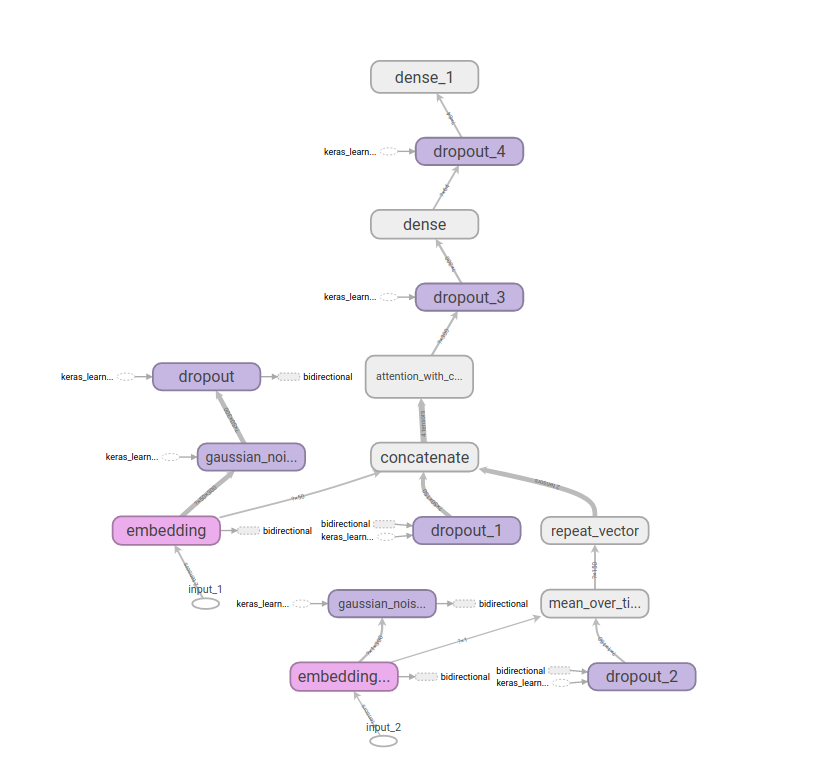
\includegraphics[width=\linewidth]{w2v_model.png}
            \caption{The model that uses Word2Vec}
            \label{fig:w2v_model}
        \end{figure}
            \begin{figure}
            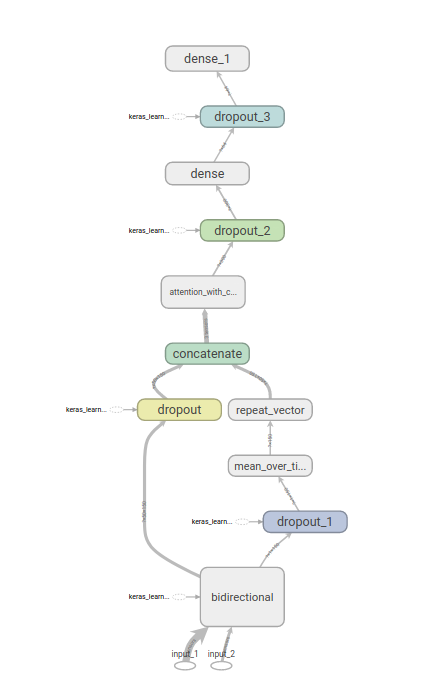
\includegraphics[width=\linewidth]{alberto_model.png}
            \caption{The model that uses AlBERTo}
            \label{fig:alberto_model}
        \end{figure}

        \subsection{ACP}\label{subsec:s1}
            Initially I only considered the positive and negative classes because of the very few mixed samples, by assigning to
            mixed reviews a random sentiment, and, although this gives nice results, I moved from a one sigmoid output neuron for
            positive and negative class, to 3 softmax output neurons for positive, negative and mixed class.
            I used class weights, which help dealing with imbalanced datasets by weighting more the misclassified prediction of a class
            with a limited number of example.
            In my case the class weights used were 1.26 for negative, 1.0 for positive and 8.14 for mixed.
            To generate the input for the model, I extracted tuples from the dataset with the form (sentiment, topic, review).
            \subsubsection{Word2Vec}
            Initially I made some experiments using a word embedding whose dimension was 128 (http://www.italianlp.it/resources/italian-word-embeddings/), but this lead to a slow and limited training, that couldn't overtake the accuracy score of 0.55, which was very bad.
            So I moved to a more informative embeddings which size is 300, and although the big dimension of 2.4GB and the poor quality of most of the entries (it is automatically generated and the quality of the words extracted from the data is very bad, lot of words are typo or sequence of random characters), it gives good results.
            The Italian Word2Vec embeddings (https://arxiv.org/pdf/2001.09332.pdf) are obtained from a simple 2-level neural network with one-hot vector as input.
            It has been trained with CBOW (continuous bag of words), the dataset was obtained using the information extracted from a dump of the Italian Wikipedia (dated 2019.04.01), from the main
categories of Italian Google News (WORLD, NATION, BUSINESS, TECHNOLOGY, ENTERTAINMENT, SPORTS, SCIENCE, HEALTH), and has dimension of 2.4 GB .
            Embeddings are given in a txt file, but after the first loading, they are formatted as dictionary and saved in a pickle file
            to speed up following loading.
            I didn't do a lot of preprocessing of the reviews, since the embedding size is big (667564 words once removed the non-ascii ones) and it could cover the 85\% of the words, but looking better at the words that were indexed as $<unk>$, a lot of them were words with a capital letter.
            So by setting all chars lowercase, without losing much information because no proper name was present in the dataset, and just by removing all \textbf{l'}, the coverage of ward embeddings increased to 95\%.
            I selected the best model by looking at the highest validation score that I obtained.
            I also tried to select the best model looking at the highest validation accuracy, but the results where something like 8 percentage points less.
            \color{orange} Orange is for train, \color{blue} blue is for validation.\color{black}
            \begin{figure}[!htb]
                \begin{minipage}{0.48\textwidth}
                    \centering
                    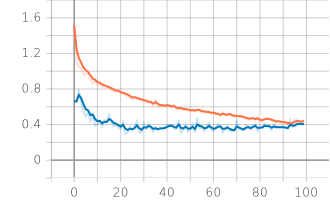
\includegraphics[width=.7\linewidth]{w2v_acp_epoch_loss.png}
                    \caption{Loss for W2V on task ACP}\label{Fig:Data1}
                \end{minipage}\hfill
                \begin{minipage}{0.48\textwidth}
                    \centering
                    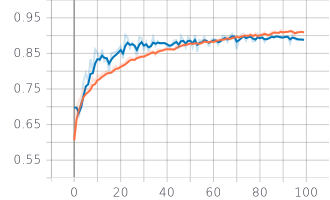
\includegraphics[width=.7\linewidth]{w2v_acp_epoch_accuracy.png}
                    \caption{Accuracy for W2V on task ACP}\label{Fig:Data2}
                \end{minipage}
                \begin{minipage}{0.48\textwidth}
                    \centering
                    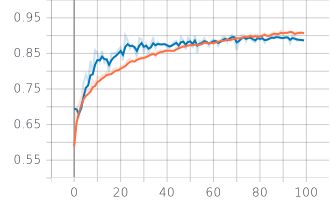
\includegraphics[width=.7\linewidth]{w2v_acp_epoch_recall.png}
                    \caption{Recall for W2V on task ACP}\label{Fig:Data3}
                \end{minipage}
            \end{figure}

            \subsubsection{AlBERTo}
            AlBERTo is the Italian BERT version.
            It has the same structure of BERT, the difference is in the learning strategy: BERT is trained with "masked learning" and "next following sentence", while alBERTo is trained only with "masked learning".
            Because of this, alBERTo is suitable for sentiment analysis tasks, but not for more complex task like QA because it does not have idea of the flow of a dialogue.
            The dataset used to train alBERTo is formed by 200 milion of tweets taken from TWITA, which is a big collection of tweets from 2012 since today.
            I used Huggingface Transformers to download alBERTo model and the tokenizer, then I decided to generate an "alBERTed" version of the dataset,
            in this way I don't need to calculate the embeddings during the training because I have already computed them,
            and this result in a faster training at the cost to spend time and space to generate and save the embedded dataset.
            The tokenizer managed to index all the words.
            The dimension of these embeddings is 768, which is much larger than the Word2Vec ones, and also this lead to better results and faster learning.
            \color{orange} Orange is for train, \color{blue} blue is for validation.\color{black}
            \begin{figure}[!htb]
                \begin{minipage}{0.48\textwidth}
                    \centering
                    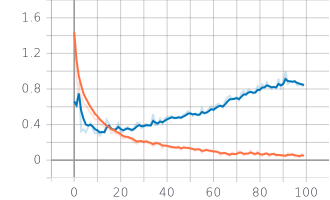
\includegraphics[width=.7\linewidth]{alberto_acp_epoch_loss.png}
                    \caption{Loss for alBERTo on task ACP}\label{Fig:Data4}
                \end{minipage}\hfill
                \begin{minipage}{0.48\textwidth}
                    \centering
                    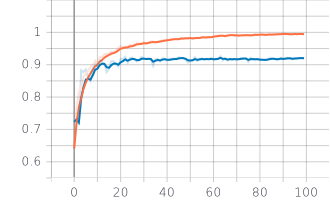
\includegraphics[width=.7\linewidth]{alberto_acp_epoch_accuracy.png}
                    \caption{Accuracy for alBERTo on task ACP}\label{Fig:Data5}
                \end{minipage}
                \begin{minipage}{0.48\textwidth}
                    \centering
                    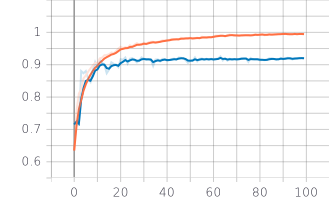
\includegraphics[width=.7\linewidth]{alberto_acp_epoch_recall.png}
                    \caption{Recall for alBERTo on task ACP}\label{Fig:Data6}
                \end{minipage}
            \end{figure}

        \subsection{ACD}\label{subsec:s2}
            Even if this model was not designed for topic-detection analysis, I experimented a way to understand its potential and limit.
            So I proceed modifying the dataset in such a way to only detect if a topic is dealt in a review, and not in which way it is dealt.
            The idea is that the context-aware attention should learn which words refers in a general way to a specific topic.
            So I tried various probability to add a negative sample (see ACD dataset description) since I obtain both class weights around 1.0, hoping that a balanced dataset could give better results.
            I also had to create negative samples for the ACD train and test set, since obviously I only had positive samples.
            In order to do so, for each review $r$ and for each absent topic $t$ I added the sample $("negative", t, r)$ with a certain probability, that I set to value 0.2.
            The approach is the same as for the ACP task, but here the output layer has dimension 1 and so has a sigmoid activation instead of a softmax.
            \color{orange} Orange is for train, \color{blue} blue is for validation.\color{black}

            \subsubsection{Word2Vec}
                The input is a list of 2 numpy array: one that contains the indexed reviews and the other one that contains the indexed topics.
                The output is a numpy array with values between [0, 1] where 0 stands for "topic not dealt in this review" and 1 stands for "topic dealt in this review.
                \begin{figure}[!htb]
                \begin{minipage}{0.48\textwidth}
                    \centering
                    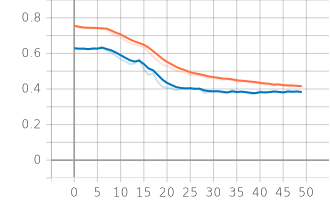
\includegraphics[width=.7\linewidth]{w2v_acd_epoch_loss.png}
                    \caption{Loss for W2V on task ACD}\label{Fig:Data7}
                \end{minipage}\hfill
                \begin{minipage}{0.48\textwidth}
                    \centering
                    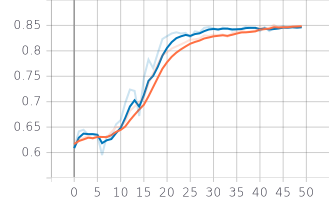
\includegraphics[width=.7\linewidth]{w2v_acd_epoch_accuracy.png}
                    \caption{Accuracy for W2V on task ACD}\label{Fig:Data8}
                \end{minipage}
                \begin{minipage}{0.48\textwidth}
                    \centering
                    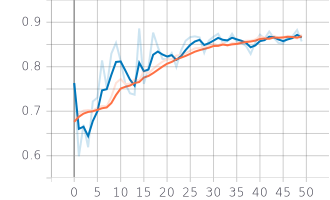
\includegraphics[width=.7\linewidth]{w2v_acd_epoch_recall.png}
                    \caption{Recall for W2V on task ACD}\label{Fig:Data9}
                \end{minipage}
            \end{figure}
            \subsubsection{AlBERTo}
                The input is a list of 2 numpy array: one that contains the embedded reviews and the other one that contains the embedded topics.
                The output is a numpy array with values between [0, 1] where 0 stands for "topic not dealt in this review" and 1 stands for "topic dealt in this review.
                \color{orange} Orange is for train, \color{blue} blue is for validation.\color{black}
                \begin{figure}[!htb]
                \begin{minipage}{0.48\textwidth}
                    \centering
                    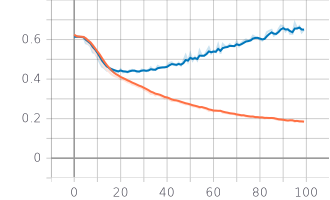
\includegraphics[width=.7\linewidth]{alberto_acd_epoch_loss.png}
                    \caption{Loss for alBERTo on task ACD}\label{Fig:Data10}
                \end{minipage}\hfill
                \begin{minipage}{0.48\textwidth}
                    \centering
                    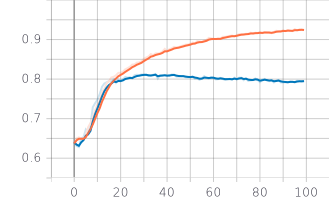
\includegraphics[width=.7\linewidth]{alberto_acd_epoch_accuracy.png}
                    \caption{Accuracy for alBERTo on task ACD}\label{Fig:Data11}
                \end{minipage}
                \begin{minipage}{0.48\textwidth}
                    \centering
                    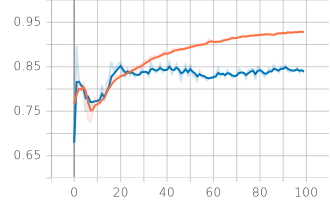
\includegraphics[width=.7\linewidth]{alberto_acd_epoch_recall.png}
                    \caption{Recall for alBERTo on task ACD}\label{Fig:Data12}
                \end{minipage}
            \end{figure}

    \section{Results}\label{sec:s5}
        I had the official gold test set during training, but I didn't use it for model selection since that would have been incorrect.
        So the model selection is based on the highest validation recall.
        I used the official evaluation\_absita script and the official gold test set for calculate the scores.
        THe official evaluation script gives us also the macro results, but the competition is based on micro measures.
        \subsection{ACD}\label{subsec:s5}
            The obvious and only way to predict the presence of topic in a sentence, is to try each topic for each sentence and collect the positive results only.
                %ACD RESULTS
                \begin{table}[h!]
                    \begin{center}
                        \caption{independent results for ACP task}
                        \label{tab:table2}
                        \begin{tabular}{l|c|c|c|r}
                            \textbf{model} & \textbf{Micro-Precision} & \textbf{Micro-Recall} & \textbf{Micro-F1-score}\\
                            \hline
                                \textbf{absita best model} & \textbf{0.8397} & \textbf{0.7837} & \textbf{0.8108}\\
                                W2V & 0.3288 & 0.3288 & 0.4745\\
                                alBERTo & 0.1604 & 0.6698 & 0.2588\\
                        \end{tabular}
                    \end{center}
                \end{table}
        As we can see, the model is not good in this task.
            \subsection{ACP}\label{subsec:s6}
            This results could be calculated in two ways: using the output of the ACD task as input, or use true topic presence information.
                In the first way, the results obviously is dependent from the result of the first task, in particular the score cannot be higher than what we obtain from the ACD task.
                So I only considered the independent tasks, because I want to consider the power of the model in the topic based sentiment analysis, and not in the aspect category detection.
                \begin{table}[h!]
                    \begin{center}
                        \caption{INDEPENDENT results for ACP task}
                        \label{tab:table4}
                        \begin{tabular}{l|c|c|r}
                            \textbf{model} & \textbf{Micro-Precision} & \textbf{Micro-Recall} & \textbf{Micro-F1-score}\\
                            \hline
                                absita best model & 0.8264 & 0.7161 & 0.7673\\
                                W2V & 0.9067 & 0.8973 & 0.9019\\
                                \textbf{alBERTo} & \textbf{0.0946} & \textbf{0.0939} & \textbf{0.0942}\\
                        \end{tabular}
                    \end{center}
                \end{table}
            We outperform the absita best model with both embeddings by a score of more than 8 percentage points, which is a huge improvement.
            The alBERTo embedding improves the results obtained by the W2V one by more than 4 percentage points, and not only has better generalization capabilities, but it learns faster.

    \section{Conclusion}\label{sec:s6}
        Deep-Learning approaches with context-attention has difficulty to understand the topics dealt in reviews.
        This could be due to a small dataset, which contains few element for each topic class.
        Simpler statistical approaches like LinearSVC gives us better results, arund 90\% for each class, thanks to lemmatization which reduces the vocabulary and has fewer elements to analyze.
        Nevertheless, the model is very good at understanding the sentiment towards a certain topic, and it can also understand if the sentiment towards a topic are mixed, and in different topics have different sentiments in the same review.
        The role of the context attention is crucial in the topic based sentiment analysis, because it can understand well which words express a certain sentiment towards a certain topic.
        Also, alBERTo embeddings are much better than W2V one, in both test results and learning speed (alBERTo started overfitting after 20 epochs, w2v after 70 epochs)
        This could depend on the bigger embedding dimension (768 vs 300), the model used to obtain them (multiple transformers vs simple neural network) and the learning strategy (CBOW vs masked learning).

\end{document}